\documentclass[11pt]{article}

\usepackage[margin=1in]{geometry}
\usepackage{amsmath,amssymb,amsthm,bm}
\usepackage{graphicx}
\usepackage{enumitem}
\usepackage{fancyhdr}
\usepackage{xcolor}
\usepackage{float}
\usepackage[hidelinks]{hyperref}

\graphicspath{{figures/}}

% ---------- Convenience macros ----------
\newcommand{\E}{\mathbb{E}}
\newcommand{\Var}{\operatorname{Var}}
\newcommand{\Prob}{P}
\newcommand{\dd}{\,\mathrm{d}}

% ---------- Environments ----------
\newenvironment{problem}[1]
{\par\bigskip\noindent\textbf{Problem #1:}\ }
{\par}
\newenvironment{solution}
{\par\medskip\noindent\textit{Solution.}\ }
{\hfill$\blacksquare$\par\medskip}

% ---------- Header ----------
\setlength{\headheight}{14pt}
\pagestyle{fancy}
\fancyhf{}
\lhead{EE 513: Stochastic Systems Theory}
\chead{Homework 3}
\rhead{Andrew Bowie}
\cfoot{\thepage}

\begin{document}

    \begin{center}
        {\Large\textbf{EE 513: Stochastic Systems Theory}}\\[2pt]
        {\large Fall 2026 \quad---\quad Prof.\ Schmid}\\[6pt]
    {\large Homework Assignment 3}\\[4pt]
        Andrew Bowie -- \LaTeX  Template by Claude\\
        Due: Thursday, October 8, 2026
    \end{center}

% =====================================================================
    \begin{problem}{3.1}
Compare the Chebychev inequality and the exact probability of the event
$\{|X - m| \ge c\}$ as a function of $c$ for
\begin{enumerate}[label=(\alph*)]
  \item $X$ is a uniform random variable in the interval $[0,1]$;
  \item $X$ is Laplacian random variable with parameter $4$;
  \item $X$ is a Gaussian random variable with mean one and variance $\sigma^2 = 16$.
  \item Find the tightest Chernoff bound on the probability of the event
  $X - m \ge c$ for the random variables in Parts (a)--(c).
\end{enumerate}
Plot your results. Display them as a function of $c$.
    \end{problem}

    \begin{solution}

        \textbf{(a)}

        The Chebyshev inequality states that
        \[
            P(|X - m| \ge k\sigma) \leq \frac{1}{k^2}
        \]
        where $k$ is the number of standard deviations away from the mean and $\sigma$ is the standard deviation.

        For a uniform random variable in the interval $[0, 1]$, $m = 0.5$.
        \begin{align*}
            Var(X) &= \frac{(b - a)^2}{12} \\
            &= \frac{1}{12} \\
            \sigma^2 &= \frac{1}{12} \\
            \sigma &= \frac{1}{\sqrt{12}}
        \end{align*}

        To compare the inequality with the event, $c = k\sigma$.
        For a given $c$, $k = \frac{c}{\sigma}$.

        Setting up the function of $c$ for $c > 0$.
        For $c \ge 0.5$, $P(|X - 0.5| \ge c) = 0$.
        For $0 < c < 0.5$:
        \begin{align*}
            f(c) &= \frac{1}{\left(\frac{c}{\sigma}\right)^2} - P(|X - 0.5| \ge c) \\
            &= \frac{1}{12c^2} - P(|X - 0.5| \ge c) \\
            &= \frac{1}{12c^2} - (1 - 2c) \quad \text{From the two edges of the bound}
        \end{align*}
        The whole function:
        \[
            f(c) = \begin{cases}
                       \frac{1}{12c^2} - (1 - 2c), & 0 < c < 0.5 \\
                       \frac{1}{12c^2} & c \geq 0.5
            \end{cases}
        \]
        Given that probabilities are $0 \leq P \leq 1$, $f(c) \geq 1$ gives us no information.
        Figure is given at the end.
        \qed

        \vspace{1em}
        \textbf{(b)}

        This assumes for the Laplacian random variable that $m = 0$ and $\lambda = 4$.
        The variance for this distribution $\sigma^2 = \dfrac{2}{\lambda^2} = \dfrac{2}{16} = \dfrac{1}{8}$, $\sigma = \dfrac{1}{\sqrt{8}}$
        Given that $m = 0$, $P(|X - m| \geq c) = P(|X| \geq c)$
        We also know that the pdf of a laplace random variable is even about its mean.
        Therefore, we can drop the absolute value and just double the total probability.
        \[
            P(|X| \geq c) = 2 \cdot P(X \geq c), c \geq 0
        \]
        That is
        \[
            2 \cdot P(X \geq c) = 2 \cdot (1 - F_X(c))
        \]
        Where
        \[
            F_X(c) = 1 - \frac{1}{2} \exp\left(-4c\right)
        \]
        Simplifying
        \begin{align*}
            2 \cdot P(X \geq c) &= 2 \cdot (1 - F_X(c)) \\
            &= 2 \cdot (1 - 1 - \frac{1}{2} \exp\left(-4c\right)) \\
            &= - \exp\left(-4c\right)
        \end{align*}

        $k = \frac{c}{\sigma}$, so $k = \frac{c}{\sigma} = c\sqrt{8}$.
        For $c > 0$:
        \begin{align*}
            f(c) &= \frac{1}{8c^2} + \exp\left(-4c\right)
        \end{align*}

        It appears that as $c \to \infty$, the bound gets tighter.
        \qed

        \vspace{1em}
        \textbf{(c)}
        $m = 1$, $\sigma = 4$
        \begin{align*}
            P(|X - 1| \geq c) &= 1 - P(X \leq 1 + c) + P(X \leq 1 - c) \\
            &= 1 - F_X(1 + c) + F_X(1 - c)
        \end{align*}
        Using a Gaussian CDF with $m = 1$, $\sigma^2 = 16$

        $c = k\sigma$, $k = \dfrac{c}{4}$, $c > 0$
        \begin{align*}
            f(c) = \dfrac{16}{c^2} -  1 + F_X(1 + c) - F_X(1 - c)
        \end{align*}

        At $c = 8$, the bound is $\dfrac{16}{64} = \dfrac{1}{4}$.
        At $c = 8$, $1 - P(X \leq 9) + P(X \leq -7) = 0.0455$, the ratio between the two is $\dfrac{1}{4\cdot0.0455} = 5.49$.
        At $c = 12$, the bound is $\dfrac{16}{144} = \dfrac{1}{9}$.
        At $c = 12$, $1 - P(X \leq 13) + P(X \leq -11) = 0.0027$, the ratio between the two is $\dfrac{1}{9\cdot0.00227} = 48.947$.

        The bound does increase with the cdf as $c \to \infty$, however it gets relatively less helpful as well.
        \qed

        \vspace{1em}
        \textbf{(d)}

        \textbf{Gaussian}

        I'll start with the Gaussian random variable.
        The characteristic function is:
        \[
            M_X(jv) = E[e^{jvX}] = \exp{\left(jmv - \dfrac{\sigma^2 v^2}{2} \right)}
        \]
        The moment generating function is related to the characteristic function by $s = jv$, $v = \dfrac{s}{j}$, $m = 1$, $\sigma^2 = 16$
        \begin{align*}
            \Phi_X(s) &= E[e^{sX}] \\
            &= \exp{\left(s - \dfrac{16 \dfrac{s^2}{j^2}}{2} \right)} \\
            &= \exp{\left(s + 8 s^2 \right)}
        \end{align*}

        For the chernoff bound:
        \begin{align*}
            P(X - m \geq c) &\leq e^{-sc} \cdot e^{-s} \cdot \Phi_X(s) \\
            &= e^{-sc} \cdot e^{-s} \cdot \exp{\left(s + 8 s^2 \right)} \\
            &= e^{-sc} \cdot \exp{\left(8 s^2 \right)} \\
            &= \exp{\left(8 s^2 -sc \right)}
        \end{align*}

        Since this is an increasing exponential, minimizing the exponent is minimizing the full equation.
        \begin{align*}
            \dfrac{d}{ds} (8 s^2 -sc) &= 16s - c \\
            \\
            \dfrac{d}{ds} (16s - c) &= 16 > 0, \quad \text{This is a minimum}
        \end{align*}

        Setting this to $0$.
        \begin{align*}
            0 &= 16s - c \\
            s &= \dfrac{c}{16}
        \end{align*}

        $s^* = \dfrac{c}{16} > 0, c > 0$
        Plugging it back in:
        \begin{align*}
            P(X - m \geq c) &\leq \exp{\left(8 (\dfrac{c}{16})^2 - c \dfrac{c}{16} \right)} \\
            P(X - m \geq c) &\leq \exp{\left(\dfrac{c^2}{32} - \dfrac{c^2}{16} \right)} \\
            P(X - m \geq c) &\leq \exp{\left(\dfrac{c^2}{32} - \dfrac{2c^2}{32} \right)} \\
            P(X - m \geq c) &\leq \exp{\left(-\dfrac{c^2}{32} \right)}
        \end{align*}

        \hrule
        \vspace{1em}

        \textbf{Laplacian}

        \[
            M_X(jv) = \frac{\alpha^2}{\alpha^2 + v^2}
        \]

        Setting up the chernoff bound, $s = jv$, $v^2 = -s^2$, $s > 0$, $\alpha = 4$
        \begin{align*}
            \phi_X(s) &= E[e^{sX}] \\
            &= \frac{16}{16 - s^2}
        \end{align*}

        To keep this defined and positive, $0 < s < 4$

        \begin{align*}
            P(X \geq c) \leq e^{-sc} \cdot \frac{16}{16 - s^2}
        \end{align*}

        Taking the natural log to simplify derivation
        \begin{align*}
            \ln{\frac{16e^{-sc}}{16 - s^2}} &= \ln{16e^{-sc}} - \ln{\left(16 - s^2\right)} \\
            &= \ln{16} - sc - \ln{\left(16 - s^2\right)} \\
            &= - sc + \ln{16} - \ln{\left(16 - s^2\right)}
        \end{align*}

        Deriving and setting equal to 0.
        \begin{align*}
            \dfrac{d}{ds} (- sc + \ln{16} - \ln{\left(16 - s^2\right)}) &= -c - \left(-2s\right) \cdot \left(\dfrac{1}{16 - s^2}\right) \\
            &= -c + \dfrac{2s}{16 - s^2} \\
            0 &= -c + \dfrac{2s}{16 - s^2} \quad \text{Set equal to 0} \\
            c &= \dfrac{2s}{16 - s^2} \\
            (16 - s^2) \cdot c &= 2s \\
            - cs^2 - 2s + 16c &= 0
        \end{align*}

        Solving with the quadratic formula
        \begin{align*}
            s &= \frac{2 \pm \sqrt{4 + 64c^2}}{-2c} \\
            &= \frac{2 \pm 2\sqrt{1 + 16c^2}}{-2c} \\
            &= \frac{1 - \sqrt{1 + 16c^2}}{-c} \quad \text{$c > 0$, so numerator must be negative} \\
            &= \frac{- 1 + \sqrt{1 + 16c^2}}{c}
        \end{align*}

        At $c = 1$, $s = - 1 + \sqrt{17}$
        As $c \to \infty$, $s = \sqrt{1 + 16c^2}{c} = 4$

        Given that this function is increasing as c increases, $s \in (0, 4)$

        Therefore
        \[
            P(X \geq c) \leq e^{-sc} \cdot \dfrac{16}{16 - s^2}
        \]
        where $s = \frac{- 1 + \sqrt{1 + 16c^2}}{c}$

        \hrule
        \vspace{1em}

        \textbf{Uniform}

        $m = 0.5$, $\sigma = \frac{1}{\sqrt{12}}$
        From the textbook,
        \[
            M_X(jv) = \frac{e^{jvb} - e^{jva}}{jv(b - a)}
        \]

        Again, $s = jv$ and $v = \frac{s}{j}$
        \begin{align*}
            \phi_X(s) &= E[e^{sX}] \\
            &= \frac{e^{sb} - e^{sa}}{s(b - a)} \\
            &= \frac{e^{s} - 1}{s}
        \end{align*}

        \begin{align*}
            P(X - \dfrac{1}{2} \geq c) &\leq e^{(-s(c + \dfrac{1}{2}))} \cdot \dfrac{e^s - 1}{s} \\
            &= e^{(-sc)}e^{\dfrac{-s}{2}} \cdot \dfrac{e^s - 1}{s}
        \end{align*}

        Taking the log and differentiating
        \begin{align*}
            \ln{\left(e^{(-sc)}e^{\dfrac{-s}{2}} \cdot \dfrac{e^s - 1}{s}\right)} &= \ln{e^{-sc}} + \ln{e^{\dfrac{-s}{2}}} + \ln{(e^s - 1)} - \ln{s} \\
            &= -sc + \dfrac{-s}{2} + \ln{(e^s - 1)} - \ln{s} \\
            & \text{Differentiating} \\
            \dfrac{d}{ds} (-sc + \dfrac{-s}{2} + \ln{(e^s - 1)} - \ln{s}) &= -c - \dfrac{1}{2} + \dfrac{e^s}{e^s - 1} - \dfrac{1}{s}
        \end{align*}

        Now optimize it by setting it to $0$
        \begin{align*}
            -c - \dfrac{1}{2} + \dfrac{e^s}{e^s - 1} - \dfrac{1}{s} &= 0 \\
            \dfrac{e^s}{e^s - 1} - \dfrac{1}{s} &= c + \dfrac{1}{2}
        \end{align*}

        This cannot be solved directly for $s$, so I'll just graph it with MATLAB

        \vspace{1em}
        \textbf{Plots.}

        \begin{figure}[H]
            \centering
            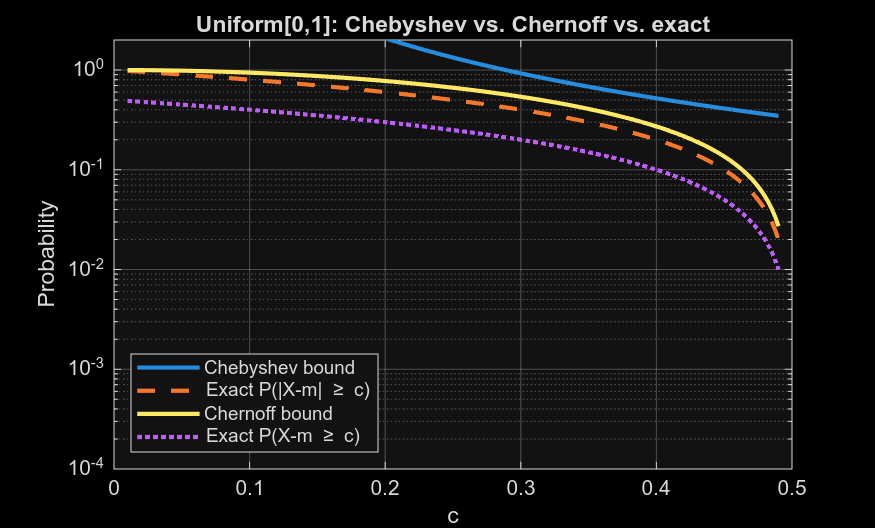
\includegraphics[width=0.38\textwidth]{3_1_a_plot}
            \caption{Plot for $f(c)$ on $0 < c < 0.5$}
        \end{figure}

        \begin{figure}[H]
            \centering
            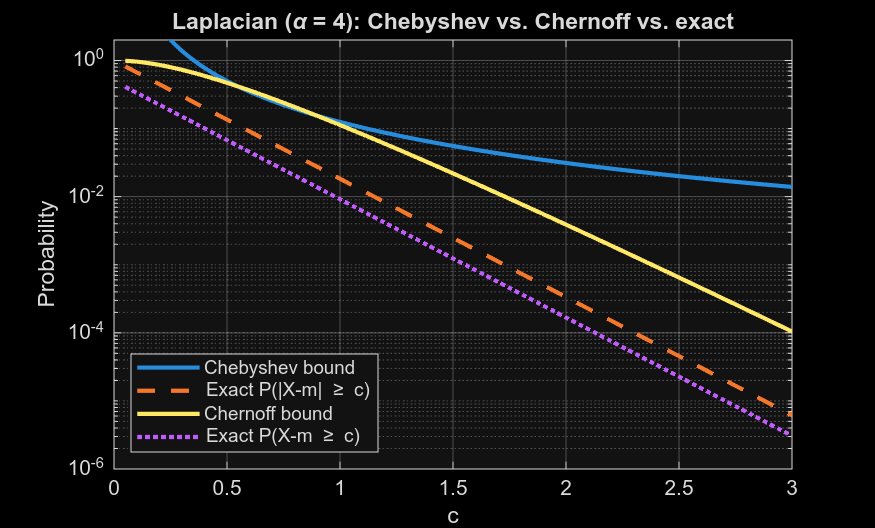
\includegraphics[width=0.38\textwidth]{3_1_b_plot}
            \caption{Plot for $f(c)$, $c > 0$}
        \end{figure}

        \begin{figure}[H]
            \centering
            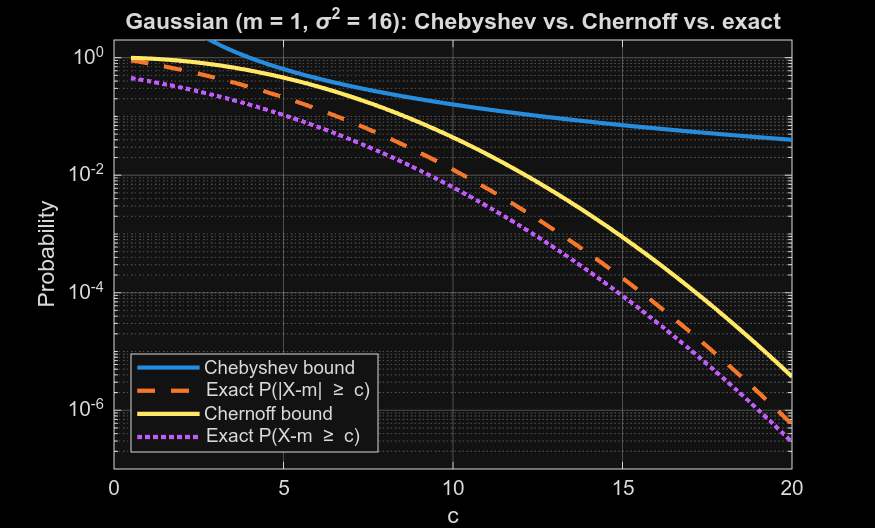
\includegraphics[width=0.38\textwidth]{3_1_c_plot}
            \caption{Plot for $f(c)$, $c > 1$}
        \end{figure}
    \end{solution}

% =====================================================================
    \begin{problem}{3.2}
Let $X$ be a discrete random variable with the following probability mass function
\[
    X = \begin{cases}
            -2, & p(-2) = 1/16\\
            -1, & p(-1) = 7/16\\
            \phantom{-}1, & p(1) = 7/16\\
            \phantom{-}2, & p(2) = 1/16
    \end{cases}
\]
\begin{enumerate}[label=(\alph*)]
  \item Find the characteristic function of the random variable,
  $M_X(jv) = E[\exp(jvX)]$.
  \item Find the entropy of the random variable.
\end{enumerate}
\textbf{\textit{Note:}} The entropy of a discrete random variable is defined as
$H(X) = E\!\left[\log_2\!\left(\frac{1}{p(X)}\right)\right]$. Entropy is known as a
measure of uncertainty in a random variable. Lossless compression is impossible
beyond the entropy limit (measured in bits per symbol).
\begin{enumerate}[label=(\alph*),start=3]
  \item Set the probability of each of the four outcomes to $1/4$. Find $H(X)$
  and compare to the result in part (b).
\end{enumerate}
    \end{problem}

    \begin{solution}
        \textbf{(a)}

        Let's set this up
        \begin{align*}
            M_X(jv) &= E[\exp(jvX)] \\
            &= \sum_{i = 1}^{4} p(X_i) \cdot \exp(jvX_i) \\
            &= \frac{1}{16} \cdot \exp(-2jv) + \frac{7}{16} \cdot \exp(-jv) + \frac{7}{16} \cdot \exp(jv) + \frac{1}{16} \cdot \exp(2jv) \\
            &= \frac{1}{16} \cdot (\cos(-2v) + j \sin(-2v)) + \frac{7}{16} \cdot (\cos(-v) + j \sin(-v)) \dots \\
            &+ \frac{7}{16} \cdot (\cos(v) + j \sin(v)) + \frac{1}{16} \cdot (\cos(2v) + j \sin(2v)) \\
            &= \frac{1}{16} \cdot (\cos(2v) - j \sin(2v)) + \frac{7}{16} \cdot (\cos(v) - j \sin(v)) \dots \\
            &+ \frac{7}{16} \cdot (\cos(v) + j \sin(v)) + \frac{1}{16} \cdot (\cos(2v) + j \sin(2v)) \\
            &= \frac{1}{16} \cdot \cos(2v) + \frac{7}{16} \cdot \cos(v) + \frac{7}{16} \cdot \cos(v) + \frac{1}{16} \cdot \cos(2v) \\
            &= \frac{1}{8} \cdot \cos(2v) + \frac{7}{8} \cdot \cos(v)
        \end{align*}

        \vspace{1em}
        \textbf{(b)}

        For entropy
        \begin{align*}
            I(X = k) &= \log_2{\dfrac{1}{P[X = k]}} = - \log_2{P[X = k]} \\
            H_X &= E[I(X)] \\
            &= - \sum_{i = 1}^{4} p(X_i) \log_2{ p(X_i) } \\
            &= - 2 (\dfrac{1}{16} \log_2{\dfrac{1}{16}} + \dfrac{7}{16} \log_2{\dfrac{7}{16}}) \\
            &= - 2 (- \dfrac{1}{16} \log_2 {16} + \dfrac{7}{16} (\log_2{7} - \log_2{16})) \\
            &= - 2 (- \dfrac{1}{16} \log_2 {16} + \dfrac{7}{16} \log_2{7} - \dfrac{7}{16} \log_2{16}) \\
            &= - 2 (\dfrac{7}{16} \log_2{7} - \dfrac{8}{16} \log_2{16}) \\
            &= - \dfrac{7}{8} \log_2{7} + 4
            &\approx 1.544
        \end{align*}

        \vspace{1em}
        \textbf{(c)}

        Setting all probabilities to $1/4$
        \begin{align*}
            H_X &= E[I(X)] \\
            &= - \sum_{i = 1}^{4} p(X_i) \log_2{ p(X_i) } \\
            &= - 4 (\dfrac{1}{4} \log_2{\dfrac{1}{4}}) \\
            &= - \log_2{\dfrac{1}{4}} \\
            &= \log_2{4} \\
            &= 2
        \end{align*}

        Comparing this to the entropy from part b, $2 > 1.544$.
        This is because by spreading out the probability uniformly, there is more uncertainty.
    \end{solution}

% =====================================================================
    \begin{problem}{3.3}
Suppose that the joint probability density function (joint pdf) for the two
random variables $X$ and $Y$ is
\[
    f_{X,Y}(x,y) = \frac{5}{12\pi}\exp\!\left[-\frac{5}{72}\left(8x^2 - 4xy + 5y^2\right)\right].
\]
\begin{enumerate}[label=(\alph*)]
  \item Determine the joint probability density function for the two random
  variables $R$ and $S$, where
  \[
      \begin{bmatrix}
                  R \\ S
      \end{bmatrix}
      = \begin{bmatrix}
                    2 & -1 \\ 1 & 2
      \end{bmatrix}
      \begin{bmatrix}
                  X \\ Y
      \end{bmatrix}.
  \]
  \item Find the following expected value $E[|2X - Y|]$.
\end{enumerate}
    \end{problem}

    \begin{solution}
        \textbf{(a)}

        We need to find the inverse of the coefficient matrix to solve for $X$ and $Y$
        \begin{align*}
            \begin{bmatrix}
                2 & -1 \\ 1 & 2
            \end{bmatrix} ^ {-1} &= \begin{bmatrix}
                2/5 & 1/5 \\
                -1/5 & 2/5
            \end{bmatrix} \\
        \end{align*}

        \begin{align*}
            \begin{bmatrix}
                R \\ S
            \end{bmatrix}
            = \begin{bmatrix}
                  2 & -1 \\ 1 & 2
            \end{bmatrix}
            \begin{bmatrix}
                X \\ Y
            \end{bmatrix}. \\
            \begin{bmatrix}
                2/5 & 1/5 \\
                -1/5 & 2/5
            \end{bmatrix} \cdot
            \begin{bmatrix}
                R \\ S
            \end{bmatrix}
            =
            \begin{bmatrix}
                X \\ Y
            \end{bmatrix}.
        \end{align*}

        Solving for $X$ and $Y$
        \begin{align*}
            X &= 2R/5 + S/5 \\
            Y &= -R/5 + 2S/5
        \end{align*}

        Calculating the jacobian
        \begin{align*}
            J &= \det \begin{bmatrix}
                    \delta r / \delta x & \delta r / \delta y \\
                    \delta s / \delta x & \delta s / \delta y
            \end{bmatrix} \\
            &= \det \begin{bmatrix}
                        2 & -1 \\
                        1 & 2
            \end{bmatrix} \\
            &= 5
        \end{align*}

        Now the joint probability $f_{R, S}(r, s)$
        \begin{align*}
            f_{R, S}(r, s) &= \frac{f_{X, Y}(2r/5 + s/5, -r/5 + 2s/5)}{5} \\
            & \text{Simplifying} \\
            &= \frac{1}{12\pi}\exp\left[-\left(\frac{r^2}{8} + \frac{s^2}{18}\right)\right] \\
            &= \frac{1}{12\pi} \exp\left[-\frac{r^2}{8}\right]\cdot \exp\left[-\frac{s^2}{18}\right]
        \end{align*}

        \vspace{1em}
        \textbf{(b)}

        Since $R = 2X - Y$, $E[|2X - Y|] = E[|R|]$.
        We need the marginal PDF of $R$, which we can find via the joint one.
        \begin{align*}
            f_R(r) &= \int_{-\infty}^{\infty} \frac{1}{12\pi} \exp\left[-\frac{r^2}{8}\right]\cdot \exp\left[-\frac{s^2}{18}\right] ds \\
            &= \frac{1}{12\pi} \exp\left[-\frac{r^2}{8}\right] \int_{-\infty}^{\infty} \exp\left[-\frac{s^2}{18}\right] ds \\
            & \text{Let $18 = 2\sigma^2$, $\sigma = 3$} \\
            &= \frac{1}{12\pi} \exp\left[-\frac{r^2}{8}\right] \int_{-\infty}^{\infty} \exp\left[-\frac{s^2}{2\sigma^2}\right] ds \\
            &= \frac{1}{\sqrt{8\pi}} \exp\left[-\frac{r^2}{8}\right] \int_{-\infty}^{\infty}  \frac{1}{\sigma\sqrt{2\pi}} \exp\left[-\frac{s^2}{2\sigma^2}\right] ds \\
            & \text{This is a Gaussian pdf, so its integral over $(-\infty, \infty)$ is $1$} \\
            &= \frac{1}{\sqrt{8\pi}} \exp\left[-\frac{r^2}{8}\right]
        \end{align*}

        Since $f_R$ is symmetric about 0, the integrand then is even, so we can just integrate the non negative numbers and double it.
        \begin{align*}
            E[|R|] &= 2 \int_{0}^{\infty} r f_R(r) dr \\
            &= \frac{2}{\sqrt{8\pi}} \int_{0}^{\infty} r \exp\left[-\frac{r^2}{8}\right] dr \\
            & u = \frac{r^2}{8}, du = \frac{r}{4} dr \\
            &= \frac{8}{\sqrt{8\pi}} \int_{0}^{\infty} \exp\left[-u\right] du \\
            &= \frac{8}{\sqrt{8\pi}} \left[-\exp[-u]\right]_{0}^{\infty} \\
            &= \frac{8}{\sqrt{8\pi}} \\
            &= \frac{\sqrt{8}}{\sqrt{\pi}}
        \end{align*}
    \end{solution}

% =====================================================================
    \begin{problem}{3.4}
Random variables $X$ and $Y$ have the following joint probability density function:
\[
    f_{X,Y}(x,y) = \begin{cases}
                       Cxe^{-xy}, & y \ge 0,\ 0 \le x \le 1\\
                       0, & \text{otherwise}
    \end{cases}
\]
The region of support for $f_{X,Y}(x,y)$ is shown below.
\begin{figure}[H]
    \centering
    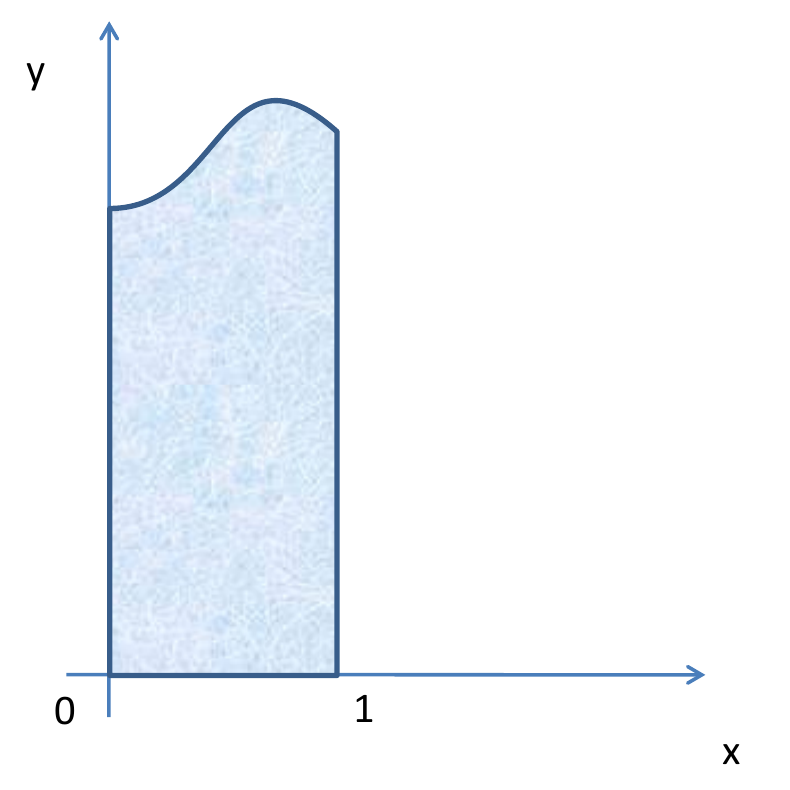
\includegraphics[width=0.38\textwidth]{fig_p34_support}
    \caption{Region of support for $f_{X,Y}(x,y)$ (Problem 3.4).}
\end{figure}
\begin{enumerate}[label=(\alph*)]
  \item Determine the constant $C$.
  \item Determine the marginal density for $Y$, and show that $E[Y]$ does not exist.
  \item Determine the marginal density for $X$.
  \item Determine the probability that $Y \le 1$.
  \item Determine the conditional density for $X$ and $Y$, given that $Y \le 1$.
  \item Determine the conditional density for $Y$, given that $X = 2$.
  \item Are $X$ and $Y$ independent? Why or why not?
  \item Determine the correlation of $X$ and $Y$ ($E[XY]$).
\end{enumerate}
\textbf{\textit{Hint:}} Use the joint pdf $f_{X,Y}(x,y)$ to solve part (d).
    \end{problem}

    \begin{solution}
        \textbf{(a)}

        Clearly we need to do a double integral over the entire range.
        \begin{align*}
            1 &= \int_{0}^{1} \int_{0}^{\infty} Cxe^{-xy} dy dx \\
            &= C \int_{0}^{1} x \int_{0}^{\infty} e^{-xy} dy dx \\
            &= C \int_{0}^{1} x \left[-\dfrac{e^{-xy}}{x}\right]_{0}^{\infty} dx \\
            &= C \int_{0}^{1} x \dfrac{1}{x} dx \\
            &= C \int_{0}^{1} 1 dx \\
            &= C \left[x\right]_{0}^{1} \\
            &= C
        \end{align*}

        We have found $C = 1$

        \vspace{1em}
        \textbf{(b)}

        We just need to integrate out x.
        \begin{align*}
            f_Y(y) &= \int_{0}^{1} x e^{-xy}\, dx
            \qquad u = x,\ du = dx,\quad dv = e^{-xy}dx,\ v = -\frac{e^{-xy}}{y} \\
            &= \left[-\frac{x e^{-xy}}{y}\right]_{0}^{1} + \frac{1}{y}\int_{0}^{1} e^{-xy}\, dx \\
            &= -\frac{e^{-y}}{y} + \frac{1}{y}\left[-\frac{e^{-xy}}{y}\right]_{0}^{1} \\
            &= -\frac{e^{-y}}{y} + \frac{1 - e^{-y}}{y^2} \\
            &= \frac{1 - e^{-y} - y e^{-y}}{y^2}, \qquad y > 0
        \end{align*}

        Expectation is
        \begin{align*}
            E[Y] &= \int_{0}^{\infty} y f_Y(y) dy \\
            &= \int_{0}^{\infty} \frac{1 - e^{-y} - y e^{-y}}{y} dy \\
            &= \int_{0}^{1} \frac{1 - e^{-y} - y e^{-y}}{y} dy + \int_{1}^{\infty} \frac{1 - e^{-y} - y e^{-y}}{y} dy \\
            &= \text{finite} + \int_{1}^{\infty} \frac{1 - e^{-y} - y e^{-y}}{y} dy
        \end{align*}

        For $y \geq 1$, $(1 + y)e^{-y}$ is decreasing, so $(1 + y)e^{-y} \leq \frac{2}{e}$ and
        \[
            1 - e^{-y} - y e^{-y} = 1 - (1 + y)e^{-y} \geq 1 - \frac{2}{e} > 0 .
        \]
        Therefore
        \begin{align*}
            \int_{1}^{\infty} \frac{1 - e^{-y} - y e^{-y}}{y}\, dy
            &\geq \left(1 - \frac{2}{e}\right) \int_{1}^{\infty} \frac{1}{y}\, dy
            = \left(1 - \frac{2}{e}\right) \Big[\ln y\Big]_{1}^{\infty} = \infty
        \end{align*}
        The integral over $[0,1]$ is finite because the integrand is bounded there
        ($y f_Y(y) \to 0$ as $y \to 0$), so $E[Y]$ diverges and does not exist.

        \qed

        \vspace{1em}
        \textbf{(c)}

        Integrate out Y
        \begin{align*}
            f_X(x) &= \int_{0}^{\infty} xe^{-xy} dy \\
            &= x \int_{0}^{\infty} e^{-xy} dy \\
            &= x \left[ -\frac{e^{-xy}}{x} \right]_{0}^{\infty} \\
            &= 1
        \end{align*}

        Note that this is only for the original range of $0 < x < 1$.
        Outside of that $f_X(x) = 0$.

        \vspace{1em}
        \textbf{(d)}

        \begin{align*}
            P(Y \leq 1) &= \int_{0}^{1} \int_{0}^{1} xe^{-xy} dy dx \\
            &= \int_{0}^{1} x \int_{0}^{1} e^{-xy} dy dx \\
            &= \int_{0}^{1} x \left[ -\dfrac{e^{-xy}}{x} \right]_0^{1} dx \\
            &= \int_{0}^{1} x \left[ -\dfrac{e^{-x}}{x} + \dfrac{1}{x} \right] dx \\
            &= \int_{0}^{1} -e^{-x} + 1 dx \\
            &= \int_{0}^{1} -e^{-x} dx + 1 \\
            &= \left[e^{-x}\right]_{0}^{1} + 1 \\
            &= \dfrac{1}{e}
        \end{align*}

        \vspace{1em}
        \textbf{(e)}

        Definition of conditional joint density
        \begin{align*}
            f_{X,Y}(x,y | A) &= \frac{f_{X, Y}(x, y)}{P(A)}
        \end{align*}
        For $(x, y) \in A$, and $0$ elsewhere

        Plugging in what we know
        \begin{align*}
            f_{X,Y}(x,y | Y \leq 1) &= \frac{f_{X, Y}(x, y)}{P(Y \leq 1)} \\
            &= e \cdot f_{X, Y}(x, y) \\
            &= \begin{cases}
                           xe^{-xy + 1}, & 0 \le y \le 1,\ 0 \le x \le 1\\
                           0, & \text{otherwise}
            \end{cases}
        \end{align*}

        \vspace{1em}
        \textbf{(f)}

        We use this definition since X can only take a single value:
        \begin{align*}
            f_{Y | X}(y | 2) &= \frac{f_{X, Y}(2, y)}{f_X(2)}
        \end{align*}
        But this doesn't exist since $f_X(2) = 0$

        \vspace{1em}
        \textbf{(g)}

        To do this, we can compare the joint function with the product of the two marginals.
        If equal, they are independent.
        \begin{align*}
            f_{X,Y}(x,y) &= f_X(x)\cdot f_Y(y) \\
            &= \frac{1 - e^{-y} - y e^{-y}}{y^2} \\
            xe^{-xy} &= \frac{1 - e^{-y} - y e^{-y}}{y^2}
        \end{align*}

        Trying at $x = 0$, $y = 1$
        \begin{align*}
            0 &= 1 - e^{-1} - e^{-1} \\
            0 &= 1 - 2e^{-1}
        \end{align*}
        This is a contradiction.
        $X, Y$ are not independent.

        \vspace{1em}
        \textbf{(h)}

        Finding the correlation:
        \begin{align*}
            E[XY] &= \int_{0}^{1} \int_{0}^{\infty} xy \cdot xe^{-xy} dy dx \\
            &= \int_{0}^{1} x^2 \int_{0}^{\infty} y \cdot e^{-xy} dy dx
        \end{align*}
        \begin{align*}
            \int_{0}^{\infty} y e^{-xy}\, dy
            \qquad u = y,\ du = dy,\quad dv = e^{-xy}dy,\ v = -\frac{e^{-xy}}{x}
        \end{align*}
        \begin{align*}
            &= \left[-\frac{y e^{-xy}}{x}\right]_{0}^{\infty} + \frac{1}{x}\int_{0}^{\infty} e^{-xy}\, dy \\
            &= 0 + \frac{1}{x}\left[-\frac{e^{-xy}}{x}\right]_{0}^{\infty} \\
            &= \frac{1}{x^2}
        \end{align*}
        \begin{align*}
            E[XY] &= \int_{0}^{1} x^2 \int_{0}^{\infty} y \cdot e^{-xy} dy dx \\
            &= \int_{0}^{1} dx \\
            &= 1
        \end{align*}
    \end{solution}

% =====================================================================
    \begin{problem}{3.5}
A communication channel called the erasure channel is shown below. Suppose that
the input symbols 0 and 1 occur with probabilities 0.4 and 0.6, respectively.
\begin{figure}[H]
    \centering
    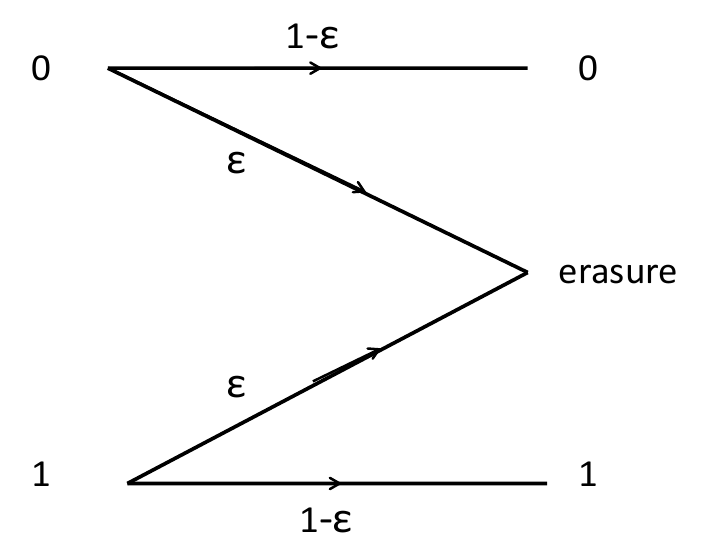
\includegraphics[width=0.45\textwidth]{fig_p35_erasure}
    \caption{Erasure channel (Problem 3.5).}
\end{figure}
\begin{enumerate}[label=(\alph*)]
  \item Find the probabilities of the output symbols (0, erasure, and 1).
  \item Suppose that a 1 is observed on the output. What is the probability that
  the input is 0? 1?
\end{enumerate}
\textbf{\textit{Comment:}} The probabilities $\varepsilon$ and $(1-\varepsilon)$ are
known as transition probabilities. These are conditional probabilities of the
outputs given the values of the inputs.
    \end{problem}

    \begin{solution}
        \textbf{(a)}

        Let's set up $X$ - Bernoulli(0.6) and $Y$ as a discrete random variable which can take values $0, 1, \text{erasure}$.

        \begin{align*}
            P(Y=0 | X=0) &= 1 - \epsilon \\
            P(Y=\text{erasure} | X = 0) &= \epsilon \\
            P(Y=1 | X=1) &= 1 - \epsilon \\
            P(Y=\text{erasure} | X = 1) &= \epsilon
        \end{align*}

        \begin{align*}
            P(Y = 1) &= P(Y=1 | X=1) \cdot P(X=1) \\
            &= (1 - \epsilon) \cdot 0.6 \\
            &= 0.6 - 0.6 \epsilon
        \end{align*}

        \begin{align*}
            P(Y = 0) &= P(Y=0 | X=0) \cdot P(X=0) \\
            &= (1 - \epsilon) \cdot 0.4 \\
            &= 0.4 - 0.4 \epsilon
        \end{align*}

        \begin{align*}
            P(Y = \text{erasure}) &= P(Y=\text{erasure} | X=0) \cdot P(X=0) + P(Y=\text{erasure} | X=1) \cdot P(X=1) \\
            &= \epsilon \cdot 0.4 + \epsilon \cdot 0.6 \\
            &= \epsilon
        \end{align*}

        \vspace{1em}
        \textbf{(b)}

        This is asking $P(X=0 | Y=1)$ and $P(X=1 | Y=1)$
        \begin{align*}
            P(X = 0 | Y = 1) &= \dfrac{P(Y = 1 | X = 0) \cdot P(X = 0)}{P(Y = 1)} \\
            &= \dfrac{0 \cdot P(X = 0)}{P(Y = 1)} \\
            &= 0
        \end{align*}
        \begin{align*}
            P(X = 1 | Y = 1) &= \dfrac{P(Y = 1 | X = 1) \cdot P(X = 1)}{P(Y = 1)} \\
            &= \dfrac{(1 - \epsilon) \cdot 0.6}{(1 - \epsilon) \cdot 0.6} \\
            &= 1 \text {If $\epsilon \in (0, 1)$}
        \end{align*}
    \end{solution}

% =====================================================================
    \begin{problem}{3.6}
Let $X$ and $Y$ be statistically independent random variables with probability
densities $f_X(x)$ and $f_Y(y)$ respectively.
\begin{enumerate}[label=(\alph*)]
  \item Let $Z = X + Y$. Demonstrate that the probability density of $Z$ is the
  convolution of the probability densities of $X$ and $Y$, and demonstrate
  that the characteristic function of $Z$ is the product of the
  characteristic functions of $X$ and $Y$.
  \item Let $W = X - Y$. Demonstrate that the probability density of $W$ is the
  correlation of the probability densities of $X$ and $Y$. Determine the
  relationship between the characteristic function of $W$ and those of
  $X$ and $Y$.
\end{enumerate}
    \end{problem}

    \begin{solution}
        \textbf{(a)}

        Let $F_Z(z) = P(X + Y \le z)$
        And let $A = \left\{ (x, y): x + y \le z \right\}$
        \begin{align*}
            F_Z(z) &= \iint_{A} f_{X, Y}(x, y) dy dx \\
            &= \iint_{A} f_X(x)f_Y(y) dy dx \quad \text{Independence} \\
            &= \int_{-\infty}^{\infty} f_X(x) \int_{-\infty}^{z - x} f_Y(y) dy dx
        \end{align*}

        Now to find $f_Z(z)$
        \begin{align*}
            f_Z(z) &= \dfrac{d}{dz} \left(\int_{-\infty}^{\infty} f_X(x) \int_{-\infty}^{z - x} f_Y(y) dy dx \right) \\
            &= \dfrac{d}{dz} \left(\int_{-\infty}^{\infty} f_X(x) F_Y(z - x) dx \right) \\
            &= \int_{-\infty}^{\infty} f_X(x) \dfrac{d}{dz} \left(F_Y(z - x)\right) dx \\
            &= \int_{-\infty}^{\infty} f_X(x) f_Y(z - x) dx \\
            &= \left( f_X * f_Y \right)(z) \\
            &= f_Z(z)
        \end{align*}

        The characteristic function is
        \begin{align*}
            M_Z(jv) &= E[e^{jvZ}] \\
            &= E[e^{jv(X + Y)}] \\
            &= E[e^{jvX + jvY}] \\
            &= E[e^{jvX}e^{jvY}] \\
            &= E[e^{jvX}]E[e^{jvY}] \quad \text{Independence} \\
            &= M_X(jv) M_Y(jv)
        \end{align*}

        \vspace{1em}
        \textbf{(b)}

        Let $F_W(w) = P(X - Y \le w)$
        And let $A = \left\{ (x, y): x - y \le w \right\}$
        \begin{align*}
            F_W(w) &= \iint_{A} f_{X, Y}(x, y) dy dx \\
            &= \iint_{A} f_X(x)f_Y(y) dy dx \quad \text{Independence} \\
            &= \int_{-\infty}^{\infty} f_Y(y) \int_{-\infty}^{w + y} f_X(x) dx dy \\
            &= \int_{-\infty}^{\infty} f_Y(y) F_X(w + y) dy
        \end{align*}

        \begin{align*}
            f_W(w) &= \dfrac{d}{dw} \left(\int_{-\infty}^{\infty} f_Y(y) F_X(w + y) dy\right) \\
            &= \int_{-\infty}^{\infty} f_Y(y) \dfrac{d}{dw} F_X(w + y) dy \\
            &= \int_{-\infty}^{\infty} f_Y(y) f_X(w + y) dy \\
            &= R_{YX}(w)
        \end{align*}

        Where $R_{YX}(w)$ is the cross correlation of $f_Y$ and $f_X$

        The characteristic function is
        \begin{align*}
            M_W(jv) &= E[e^{jvW}] \\
            &= E[e^{jv(X - Y)}] \\
            &= E[e^{jvX - jvY}] \\
            &= E[e^{jvX}e^{-jvY}] \\
            &= E[e^{jvX}]E[e^{-jvY}] \quad \text{Independence} \\
            &= E[e^{jvX}]E[e^{j(-v)Y}] \\
            &= M_X(jv)M_Y(-jv)
        \end{align*}

        \begin{align*}
        \end{align*}

    \end{solution}

% =====================================================================
    \begin{problem}{3.7 (Leon-Garcia, Problem 154, p.\ 189)}
The random variable $X$ is uniformly distributed in the interval $[0,a]$. Suppose
$a$ is unknown, so we estimate $a$ by the maximum value observed in $n$
independent repetitions of the experiment; that is, we estimate $a$ by
$Y = \max\{X_1, X_2, \ldots, X_n\}$.
\begin{enumerate}[label=(\alph*)]
  \item Find $P[Y \le y]$.
  \item Find the mean and variance of $Y$, and explain why $Y$ is a good estimate
  for $a$ when $n$ is large.
\end{enumerate}
    \end{problem}

    \begin{solution}
        \textbf{(a)}

        This is a continuous, not a discrete, random variable.
        This is, in effect
        \begin{align*}
            P[Y \le y] &= P[\max\{X_1, X_2, \ldots, X_n\} \le y] \\
            &= P[X_1 \le y \cap X_2 \le y \cap \ldots \cap X_n \le y] \\
            &= P[X_1 \le y] \cdot P[X_2 \le y] \cdot \ldots \cdot P[X_n \le y] \quad \text{Independence}
        \end{align*}
        For any of these, $P[X_i \le y] = \min\{\dfrac{y}{a}, 1\}$, for $y \ge 0$
        So together
        \begin{align*}
            P[Y \le y] &= P[X_1 \le y] \cdot P[X_2 \le y] \cdot \ldots \cdot P[X_n \le y] \\
            &= \min\{\dfrac{y^n}{a^n}, 1\}
        \end{align*}

        All together
        \[
            F_Y(y) = P[Y \le y] = \begin{cases}
                             0, & y < 0 \\
                             \left(\dfrac{y}{a}\right)^n, & 0 \le y \le a \\
                             1, & y > a
            \end{cases}
        \]

        \vspace{1em}
        \textbf{(b)}

        First we need to find $f_Y$, for $0 \le y \le a$
        \begin{align*}
            f_Y(y) &= \dfrac{d}{dy} \left(\dfrac{y}{a}\right)^n \\
            &= \dfrac{ny^{n-1}}{a^n}
        \end{align*}

        Now that we have $f_Y$
        \begin{align*}
            E[Y] &= \int_{0}^{a} y \cdot f_Y(y) dy \\
            &= \int_{0}^{a} y \cdot \dfrac{ny^{n-1}}{a^n} dy \\
            &= \int_{0}^{a} \dfrac{ny^n}{a^n} dy \\
            &= \dfrac{n}{a^n} \int_{0}^{a} y^n dy \\
            &= \dfrac{n}{a^n} \left[ \dfrac{y^{n + 1}}{n + 1} \right]_{0}^{a} \\
            &= \dfrac{n}{a^n} \left[ \dfrac{a^{n + 1}}{n + 1} \right] \\
            &= \dfrac{n}{a^n} \dfrac{a^{n + 1}}{n + 1} \\
            &= \dfrac{an}{n + 1}
        \end{align*}
        \begin{align*}
            E[Y^2] &= \int_{0}^{a} y^2 \cdot f_Y(y) dy \\
            &= \int_{0}^{a} y^2 \cdot \dfrac{ny^{n-1}}{a^n} dy \\
            &= \int_{0}^{a} \dfrac{ny^{n + 1}}{a^n} dy \\
            &= \dfrac{n}{a^n} \int_{0}^{a} y^{n + 1} dy \\
            &= \dfrac{n}{a^n} \left[ \dfrac{y^{n + 2}}{n + 2} \right]_{0}^{a} \\
            &= \dfrac{n}{a^n} \left[ \dfrac{a^{n + 2}}{n + 2} \right] \\
            &= \dfrac{n}{a^n} \dfrac{a^{n + 2}}{n + 2} \\
            &= \dfrac{a^2 n}{n + 2}
        \end{align*}
        \begin{align*}
            E[Y] &= \dfrac{an}{n + 1} \\
            Var(Y) &= E[Y^2] - (E[Y])^2 \\
            &= \dfrac{a^2 n}{n + 2} - \dfrac{a^2 n^2}{(n + 1)^2}
        \end{align*}

        As $n \to \infty$
        \begin{align*}
            \lim_{n \to \infty} E[Y] &= \lim_{n \to \infty} \dfrac{an}{n + 1} \\
            &= a \cdot \lim_{n \to \infty} \dfrac{n}{n + 1} \\
            &= a
        \end{align*}
        \begin{align*}
            \lim_{n \to \infty} Var(Y) &= \lim_{n \to \infty} \dfrac{a^2 n}{n + 2} - \dfrac{a^2 n^2}{(n + 1)^2} \\
            &= a^2 \cdot \lim_{n \to \infty} \dfrac{n}{n + 2} - a^2 \cdot \lim_{n \to \infty} \dfrac{n^2}{(n + 1)^2} \\
            &= a^2 - a^2 \\
            &= 0
        \end{align*}

        Since $E[Y] \to a$ and $\mathrm{Var}(Y) \to 0$ as $n \to \infty$, $Y$ concentrates
        at $a$, so $Y$ is a good estimate of $a$ when $n$ is large.

    \end{solution}

% =====================================================================
    \begin{problem}{3.8}
Let $Y = X_1 + X_2 + \cdots + X_n$, where $X_i$ are mutually independent random
variables. Using the relationship between the characteristic function $M_Y(jv)$
and probability density function $f_Y(y)$ of random variable $Y$ prove the
following results:
\begin{enumerate}[label=(\alph*)]
  \item Suppose that $X_i$ is normally distributed $N(m_i, \sigma_i^2)$ for each $i$.
  Show that $Y$ is also normally distributed with mean $\sum_{i=1}^n m_i$
  and variance $\sum_{i=1}^n \sigma_i^2$.
  \item Suppose that $X_i$ is Poisson distributed with parameter $\lambda_i$ for
  each $i$; that is,
  \[
      \Pr(X_i = k) = \frac{\lambda_i^k}{k!}e^{-\lambda_i}.
  \]
  Show that $Y$ is also Poisson distributed with parameter
  $\sum_{i=1}^n \lambda_i$.
  \item Suppose that $X_i$ is Cauchy distributed with parameters $a_i$ and $b_i$
  for each $i$; that is,
  \[
      f_{X_i}(x) = \frac{1}{\pi b_i}\left(1 + \frac{(x - a_i)^2}{b_i^2}\right)^{-1}.
  \]
  Show that $Y$ is also Cauchy distributed with parameters
  $a_Y = \sum_{i=1}^n a_i$ and $b_Y = \sum_{i=1}^n b_i$.
  \item Suppose that $X_i$ is chi-square with $N_i$ degrees of freedom for each
  $i$; that is,
  \[
      f_{X_i}(x) = \frac{x^{\left(\frac{N_i}{2}\right)-1}}
      {2^{\left(\frac{N_i}{2}\right)}\sigma^{N_i}\,\Gamma\!\left(\frac{N_i}{2}\right)}
      \, e^{-\frac{x}{2\sigma^2}}\, u(x),
  \]
  where $u(x) = 1$, for $x \ge 0$, and $u(x) = 0$, otherwise. Show that $Y$
  is also chi-square with $N_Y = \sum_{i=1}^n N_i$ degrees of freedom.
\end{enumerate}
\textbf{\textit{Note:}} probability density functions preserved under summation
are called \emph{reproducing densities}. So, the normal, Poisson, Cauchy, and
chi-square densities are all examples of reproducing densities.
    \end{problem}

    \begin{solution}
        \textbf{(a)}

        \begin{align*}
            M_Y(jv) &= E[e^{jvY}] \\
            &= E[e^{jv(X_1 + X_2 + \cdots + X_n)}] \\
            &= E[e^{jvX_1}e^{jvX_2} \ldots e^{jvX_n}] \\
            &= E[e^{jvX_1}]E[e^{jvX_2}] \ldots E[e^{jvX_n}] \quad \text{Independence} \\
            &= M_{X_1}(jv)M_{X_2}(jv) \ldots M_{X_n}(jv)
        \end{align*}

        For each $X_i$ Gaussian random variable with mean $m_i$ and variance $\sigma_i^2$
        \begin{align*}
            M_{X_i}(jv) &= \exp\left(jv m_i - \dfrac{\sigma_{i}^{2}v^2}{2}\right)
        \end{align*}

        \begin{align*}
            M_Y(jv) &= M_{X_1}(jv)M_{X_2}(jv) \ldots M_{X_n}(jv) \\
            &= \prod_{i=1}^{n} \exp\left(jv m_i - \dfrac{\sigma_{i}^{2}v^2}{2}\right) \\
            &= \exp\left(jv (\sum_{i=1}^{n} m_i) - \dfrac{ v^2 \sum_{i=1}^{n} \sigma_{i}^{2} }{2}\right)
        \end{align*}

        This shows that the characteristic function of $Y$ is the characteristic function of a Gaussian random variable with mean $\sum_{i=1}^{n} m_i$ and variance $\sum_{i=1}^{n} \sigma_{i}^{2}$

        \vspace{1em}
        \textbf{(b)}

        Using the same derivation of characteristic functions from above,
        \begin{align*}
            M_Y(jv) &= M_{X_1}(jv)M_{X_2}(jv) \ldots M_{X_n}(jv) \\
            &= \prod_{i=1}^{n} \exp{\left( \lambda_i (e^{jv} - 1) \right)} \\
            &= \exp{\left( ( \sum_{i = 1}^{n} \lambda_i) (e^{jv} - 1) \right)}
        \end{align*}

        This lines up with the characteristic function of the poisson random variable with parameter $\sum_{i = 1}^{n} \lambda_i$

        \vspace{1em}
        \textbf{(c)}

        I will follow the same reasoning.
        \begin{align*}
            M_Y(jv) &= M_{X_1}(jv)M_{X_2}(jv) \ldots M_{X_n}(jv) \\
            &= \prod_{i=1}^{n} \exp{\left( jva_i - b_i |v| \right)} \\
            &= \exp{\left( jv (\sum_{i = 1}^{n} a_i) - (\sum_{i = 1}^{n} b_i) |v| \right)}
        \end{align*}

        In this case, this is a Cauchy random variable with parameters $\sum_{i = 1}^{n} a_i$ and $\sum_{i = 1}^{n} b_i$

        \vspace{1em}
        \textbf{(d)}

        Following the same reasoning
        \begin{align*}
            M_Y(jv) &= M_{X_1}(jv)M_{X_2}(jv) \ldots M_{X_n}(jv) \\
            &= \prod_{i=1}^{n}\left( 1 - 2jv \sigma^2 \right)^{-N_i/2} \\
            &= \left( 1 - 2jv \sigma^2 \right)^{-\dfrac{1}{2}(\sum_{i = 1}^{n} N_i) }
        \end{align*}

        Which matches a chi square random variable with $\sum_{i = 1}^{n} N_i$ degrees of freedom.

    \end{solution}

\end{document}
